\subsection{Entity-Relationship Schema}

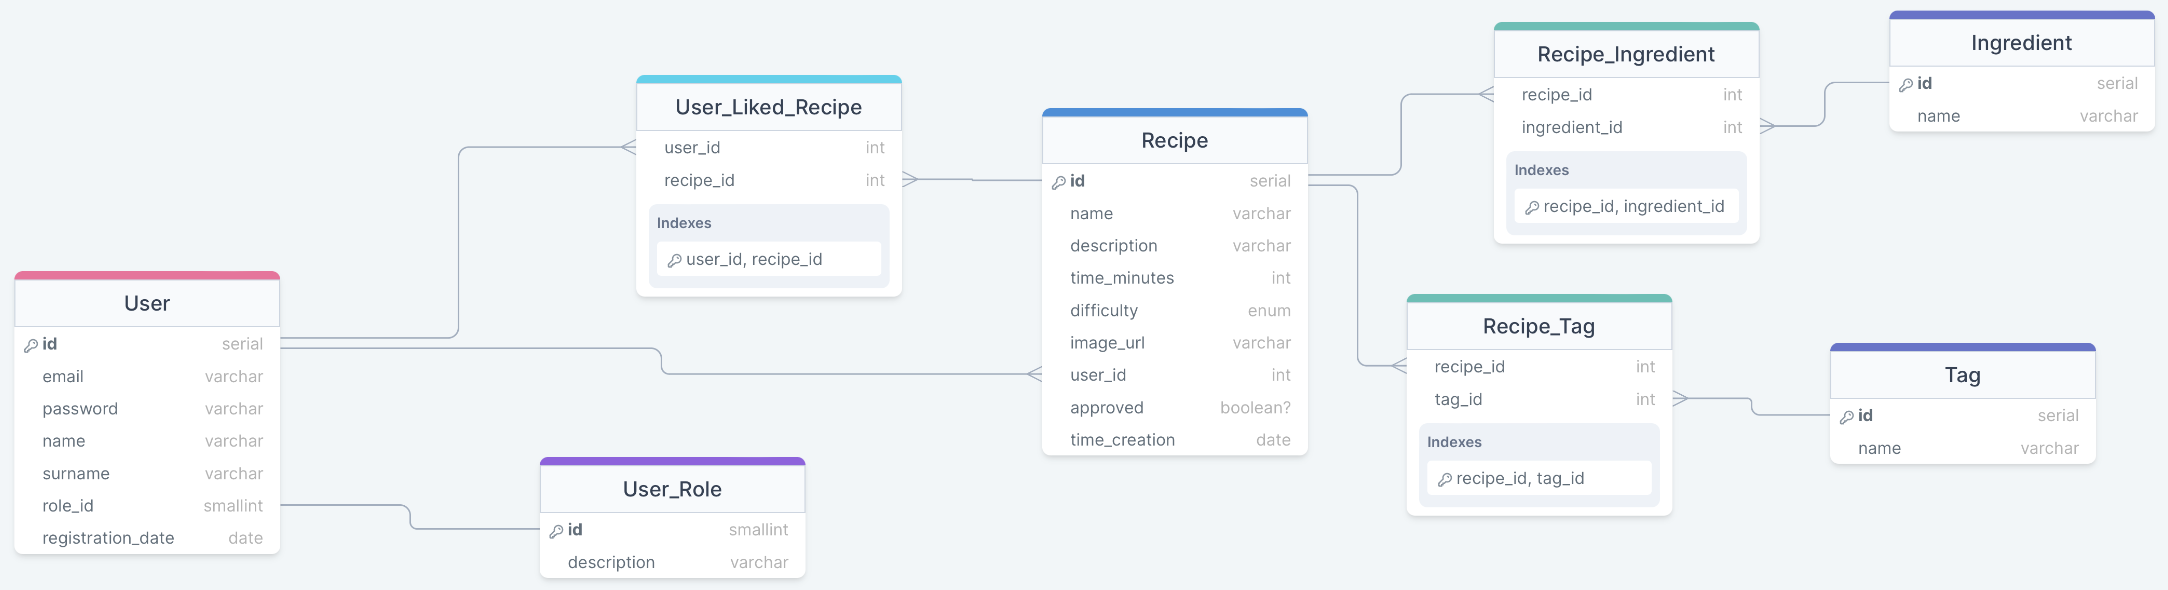
\includegraphics[width=\textwidth]{images/er.png}

The following is the description of the ER Schema of the database (PostgreSQL) for the web app.\\

\begin{itemize}
    \item \textbf{User}: Represents users of the website.
    \begin{itemize}
        \item \underline{id} (primary key): INTEGER - the serial id associated to the user
        \item email: VARCHAR(255) - user's email
        \item password: VARCHAR(255) - user's password, hashed using SHA256
        \item name: VARCHAR(255) - user's name
        \item surname: VARCHAR(255) - user's surname
        \item role\_id (foreign key referencing User\_Role): SMALLINT - the role of the user
        \item registration\_date: DATE - user's registration date
    \end{itemize}
    
    \item \textbf{User\_Role}: Describes the 5 defined roles that users can have: "admin", "user", "banned", "unverifiedUser" and "unverifiedAdmin"
    \begin{itemize}
        \item \underline{id} (primary key): SMALLINT - id of the rol
        \item description: VARCHAR(255) - title of the role
    \end{itemize}
    
    \item \textbf{Recipe}: Stores information about recipes.
    \begin{itemize}
        \item \underline{id} (primary key): SERIAL - serial id of the recipe
        \item name: VARCHAR(255) - recipe's title
        \item description: VARCHAR(255) - description/preparation of the recipe
        \item time\_minutes: INTEGER - time needed for the preparation of the recipe (in minutes)
        \item difficulty: VARCHAR(255) - enumerator for the difficulty of the recipe: "easy", "medium", "hard"
        \item image\_url: VARCHAR(255) - url for a thumbnail image of the recipe
        \item user\_id (foreign key referencing User): INTEGER - id of the user that created the recipe
        \item approved: BOOLEAN - value that represents the status of the recipe: "NULL" = to be approved, "true" = approved, "false" = not approved
        \item time\_creation: DATE - date of creation of the recipe
    \end{itemize}
    We chose to keep the URL of the image in the database instead of directly memorizing the image to balance the memory load of the site (for wich we are billed by the provider of the site) and to allow an easier portability ,recostruction and modification of the schema. This does not create any issues since, even if users input harmful or not appropriate data in a Recipe, it will not get approved and eventually will get deleted.


      \item \textbf{Ingredient}: Contains information about ingredients.
    \begin{itemize}
        \item \underline{id} (primary key): SERIAL - serial id of the ingredient
        \item name: VARCHAR(255) - name of the ingredient
    \end{itemize}

        \item \textbf{Recipe\_Ingredient}: Represents the ingredients used in recipes.
    \begin{itemize}
        \item \underline{recipe\_id} (foreign key referencing Recipe): INTEGER - id of the recipe
        \item \underline{ingredient\_id} (foreign key referencing Ingredient): INTEGER - id of the ingredient
    \end{itemize}
    This table is used for the many-to-many relationship between recipes and ingredients, indicating which ingredients are used in each recipe.
    

      \item \textbf{Tag}: Contains information about tags that can be associated with recipes.
    \begin{itemize}
        \item \underline{id} (primary key): SERIAL - id of the tag
        \item name: VARCHAR(255) - name of the tag
    \end{itemize}
    
    
    \item \textbf{Recipe\_Tag}: Links recipes to tags.
    \begin{itemize}
        \item \underline{recipe\_id} (foreign key referencing Recipe): INTEGER - id of the recipe
        \item \underline{tag\_id} (foreign key referencing Tag): INTEGER - id of the tag
    \end{itemize}
    This table is used to associate multiple tags with multiple recipes.
    
  
    \item \textbf{User\_Liked\_Recipe}: Tracks which recipes users have liked.
    \begin{itemize}
        \item \underline{user\_id} (foreign key referencing User): INTEGER - id of the user
        \item \underline{recipe\_id} (foreign key referencing Recipe): INTEGER - id of the recipe
    \end{itemize}
    This table facilitates the many-to-many relationship between users and recipes specifying which recipes each user has liked.
    

  
\end{itemize}

Foreign key constraints ensure referential integrity between related tables and primary keys uniquely identify records within each table.
